\lecture{Фильтры и классические растровые задачи}{Юля Кононова}

\subsection{Фильтры}
\paragraph{Ядро свертки}
Ядро свёртки~--- это небольшая матрица чисел, которая используется для выполнения математических операций над изображением. При свёртке изображения с ядром, каждое значение пикселя заменяется взвешенной суммой соседних пикселей, где веса задаются элементами ядра.
\paragraph{Как работает свёртка?}

\begin{figure}[h]
    \centering
    \includesvg[inkscapelatex=false, width=0.5\textwidth]{kernel}
    \caption{Пример применения фильтра к изображению}
    \label{fig:kernel}
\end{figure}

\begin{enumerate}
    \item Ядро накладывается на часть изображения (размер накладываемой области равен размеру ядра) (Рис.~\ref{fig:kernel});
    \item Значения пикселей из изображения умножаются на соответствующие элементы ядра;
    \item Полученные результаты суммируются (Рис.~\ref{fig:kernel_2}), и итоговое значение записывается в соответствующий пиксель новой (результирующей) матрицы;
    \item Ядро сдвигается по всему изображению, пока операция не будет выполнена для всех пикселей.
\end{enumerate}

\begin{figure}[h]
    \centering
    \includesvg[inkscapelatex=false, width=0.5\textwidth]{kernel2}
    \caption{Пример математических вычислений, выполненных для одного пикселя. Для примера, показанного на Рис. 1, пиксель со значением $e$ меняет свое значение следующим образом.}
    \label{fig:kernel_2}
\end{figure}

\subsubsection{Контрастно повышающий фильтр}

\begin{figure}[h]
    \centering
    \includesvg[inkscapelatex=false, width=0.5\textwidth]{sharpen_filter}
    \caption{Примеры ядра свертки для контрастно повышающего фильтра}
    \label{fig:sharpen_filter}
\end{figure}

Контрастно повышающий фильтр представляет собой один из методов обработки изображений, применяемый для выделения деталей и улучшения его визуального восприятия. Данный фильтр работает путем усиления контраста между соседними пикселями, делая различия между светлыми и тёмными областями более выраженными. В рамках цифровой обработки изображений контрастное повышение зачастую реализуется с использованием операции свёртки. Для этой цели применяются специальные свёрточные ядра, которые акцентируют внимание на разнице между центральным пикселем и его соседями. Примеры таких свёрточных ядер можно увидеть на Рис.~\ref{fig:sharpen_filter}.

Для более детального рассмотрения процесса усиления контраста возьмем вторую матрицу с Рис.~\ref{fig:sharpen_filter} и обратим внимание на ситуацию, возникающую на границе двух областей с различной интенсивностью. Рассмотрим пример, когда в процессе свёртки мы находимся на границе областей с яркостью $Y$ и $X$, где $Y$ существенно меньше $X$ ($Y<<X$). В этом случае изменение цвета для точек $A$ и $B$ будет происходить следующим образом:
\\
\begin{figure}[h]
    \centering
    \includesvg[inkscapelatex=false, width=0.5\textwidth]{sharpen_on_border}
    \caption{Изменение яркости цветов на границе}
    \label{fig:sharpen_on_border}
\end{figure}
\\

Разница в цвете изменится в 7 раз:
\begin{itemize}
    \item Старая разница в яркости между $X$ и $Y$:
          \[\Delta = X - Y\]
    \item Новая разница в яркости:
          \[\tilde \Delta= 7X - 7Y = 7(X - Y)\]
\end{itemize}

Внутри области цвета $X$ и $Y$ яркости и цвета не изменятся.\\

Общий вид таких матриц представлен на Рис.~\ref{fig:sharpen_general_view}.
\\
\begin{figure}[h]
    \centering
    \includesvg[inkscapelatex=false, width=0.5\textwidth]{sharpen_general_view}
    \caption{Общий вид ядра свертки для контрастно повышающего фильтра}
    \label{fig:sharpen_general_view}
\end{figure}
\\

Управляя $\alpha$ и $\beta$ можем контролировать контрастность.

Если контрастность выкрутить на полную (поставить вместо $\alpha$ и $\beta$ очень большие числа), то получим черно-белую картинку.
Бледные цвета станут белыми. Яркие~-- черными.

\subsection{Задача определения границ и выделения сегментов}

Граница~--- перепад цветов.

Для ее определения можно посчитать градиент яркости изображения.

Градиент представляет собой вектор, характеризующий направление наибольшего изменения интенсивности, а его величина указывает на скорость этого изменения. Высокие значения градиента соответствуют резким перепадам яркости, что, как правило, указывает на наличие границ.

В подсчета градиента помогает дискретный дифференциальный оператор~--- оператор Собеля.
\paragraph{Оператор Собеля}

\begin{figure}[h]
    \centering
    \includesvg[inkscapelatex=false, width=0.7\textwidth]{sobel}
    \caption{Оператор Собеля}
    \label{fig:sobel}
\end{figure}

Оператор Собеля~--- линейный оператор размера 3$\times$3. Он смотрит как идет перепад яркости одного из цветов по горизонтали и по вертикали. Поэтому на самом деле есть два симметричных оператора по x (по горизонтали) и по y (по вертикали). Они представлены на Рис.~\ref{fig:sobel}.

Важно учитывать, что результат, полученный после применения такого фильтра~--- это не есть изображение, а скорее карта перепада цветов. С примером работы фильтра можно ознакомиться на Рис.~\ref{fig:sobel_example}.

\begin{figure}[h]
    \centering
    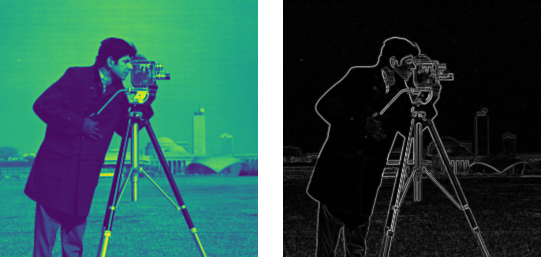
\includegraphics[width=0.5\textwidth]{sobel_example.png}
    \caption{Пример работы оператора Собеля}
    \label{fig:sobel_example}
\end{figure}

Рассмотрим ситуацию на границе двух цветов разной яркости $Y$ и $X$, где $Y$ существенно меньше $X$ ($Y<<X$). После применения ядра свертки $G_x$ изменение цвета для точек $A$ и $B$ можно увидеть на Рис.~\ref{fig:sobel_on_border}.

\begin{figure}[h]
    \centering
    \includesvg[inkscapelatex=false, width=0.5\textwidth]{sobel_on_border}
    \caption{Изменение яркости цветов на границе для оператора Собеля}
    \label{fig:sobel_on_border}
\end{figure}

Применяя фильтр на не граничные пиксели, будем получать 0:
\[
    G_x|_{пиксель \ внутри \  одной \ области}= 0
\]

После применения $G_y$ будем получать изменения по вертикали.

Можно явно понимать в какую сторону по горизонтали и по вертикали растет значение цвета, зафиксировав, что положительные значения означают убывание яркости по горизонтали слева направо, отрицательные~--- возрастание.

Свертка изображения $Img$ с этими ядрами дает две карты градиентов:
\[
    G_x(Img) = \frac{d Br}{dx} (x)
\]
\[
    G_y(Img) = \frac{d Br}{dy} (y)
\]

Их можно использовать, чтобы найти абсолютную величину градиента в каждой точке($G$) и его направление(в какую сторону яркость растет сильнее всего)($\theta$):
\[
    G = \sqrt{G_x^2 + G_y^2} = |\triangledown Br|
\]

\[
    \theta = arctg \frac{G_x}{G_y}
\]

Это значит, что для каждой точки можно понять в какую сторону и с какой силой растет яркость.

Таким образом оператор Собеля позволяет получить два представления градиента:
\begin{itemize}
    \item В декартовой системе: горизонтальные (\(G_x\)) и вертикальные (\(G_y\)) изменения.
    \item В полярной системе: величина (\(G\)) и направление (\(\theta\)) градиента.
\end{itemize}

Эти представления эквивалентны и могут быть использованы в зависимости от задачи.

Для корректной обработки изображения граничные пиксели (самые верхние, нижние, левые и правые строки) исключаются, так как их вычисление нарушает гладкость результатов.

\subsection{Нелинейные фильтры}
В отличие от линейных фильтров, которые используют операции свёртки, нелинейные фильтры обрабатывают изображение на основе нелинейных преобразований.
\\

Примеры:
\begin{enumerate}
    \item Медианный фильтр~--- альтернативный сглаживающий фильтр. Для каждой точки изображения значение пикселя заменяется на медиану значений в её локальном окне (например, 3×3 или 5×5 пикселей).
    \item Пороговый фильтр~--- фильтр, используемый для бинаризации изображения, то есть для преобразования его в чёрно-белый формат на основе порогового значения. Если значение пикселя превышает заданное пороговое значение, то пикселю присваивается значение 1, меньше~--- 0.
\end{enumerate}

\subsection{Классические растровые задачи}
К классическим растровым задачам относятся:
\begin{enumerate}
    \item Задача векторизации
    \item Задача сегментации
\end{enumerate}

\subsection{Задача векторизации}
Векторизация~--- процесс преобразования растрового изображения (набор пикселей) в векторное представление (набор объектов).

Принцип работы: Идентификация границ в растровом изображении и их аппроксимация геометрическими примитивами.

С  помощью предыдущего алгоритма можно выделить границы объектов. А как понять, что объект единый? Помогает волновой алгоритм.

\paragraph{Волновой алгоритм}
Задача алгоритма: выделить на изображении однородные области, которые впоследствии будут преобразованы в векторные примитивы.
\\

Принцип работы:
\begin{enumerate}
    \item Берутся опорные точки;
    \item Волновым образом алгоритм проходится по соседним пикселям, проверяя изменение цвета (попадает ли новый пиксель в интервал возможных значений данной области). Если проверка пройдена пиксели объединяются в одну область;
    \item В итоге окажется выделен сегмент, который можно считать отдельным примитивом.
\end{enumerate}

Рассмотрим на примере. На Рис.~\ref{fig:line} меткой показана опорная точка. За 3 шага выполняется обход объекта и в итоге выделяется примитив.

\begin{figure}[h]
    \centering
    \includesvg[inkscapelatex=false, width=0.8\textwidth]{line}
    \caption{Пример работы волнового алгоритма}
    \label{fig:line}
\end{figure}

Как из полученной фигуры понять примитив? В этом может помочь скелетный метод.

\paragraph{Построение скелета изображения}
Если есть фигура можно построить по ней скелет.

Скелет~--- набор отрезков, который сохраняет топологические свойства исходного объекта, такие как связность и количество компонентов, но при этом существенно упрощает его геометрическое представление. Скелет можно рассматривать как своего рода аналог полигональной сетки для трёхмерных изображений.
\\

Алгоритм построения:
\begin{enumerate}
    \item Исходной границей объекта считается его контур;
    \item Границы объекта начинают двигаться внутрь с одинаковой скоростью, перпендикулярно своим направлениям;
    \item В процессе движения фиксируются траектории точек пересечения сторон границы. Эти траектории определяются биссектрисами углов между сторонами;
    \item Если в процессе сжатия происходит полное исчезновение (схлопывание) какого-либо сегмента до нулевой длины, траектория продолжается под другим углом. Такие изменения фиксируются и добавляются в структуру скелета;
    \item Процесс продолжается до тех пор, пока объект не будет полностью преобразован в скелет, состоящий из отрезков.
\end{enumerate}

С примером работы алгоритма можно ознакомиться на Рис.~\ref{fig:skeleton}.

\begin{figure}[h]
    \centering
    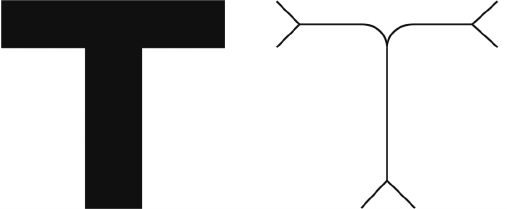
\includegraphics[width=0.5\textwidth]{skeleton.png}
    \caption{Пример работы скелетного метода}
    \label{fig:skeleton}
\end{figure}

Результатом построения скелета является набор отрезков с заданными характеристиками, такими как цвет и толщина. Толщина линий скелета определяется количеством шагов, сделанных алгоритмом от границы объекта внутрь. Процесс можно представить как волновой алгоритм, где волны распространяются от внешней границы объекта к его центру. Таким образом, толщина линий скелета отражает глубину расположения соответствующих элементов относительно исходной границы.

После этого можно использовать различные оптимизации скелета.
Скелет представляется в виде набора коротких отрезков, которые приближённо воспроизводят его форму. Поэтому можно использовать:
\begin{itemize}
    \item Построение кривых Безье:

          Если граница имеет криволинейную форму, строится кривая Безье. Особенно полезны для описания скруглённых форм и плавных переходов.
    \item Регрессионные оценки:

          Если набор отрезков можно описать одной прямой (например, его точки лежат близко к линии), то он представляется как единая линия.
\end{itemize}

И таким образом по чуть-чуть разбирается изображение.

\subsection{Задача сегментации}
Сегментация изображения является одной из ключевых задач в области обработки и анализа изображений, особенно на этапе их предобработки. Основная цель сегментации заключается в разделении изображения на отдельные области по какому-то признаку.

Существует множество подходов к решению задачи сегментации, каждый из которых основан на различных принципах и алгоритмах. Основные из них включают:

\begin{enumerate}
    \item Алгоритмические методы (например, волновой алгоритм). Хуже всего работает в плане надежности, но при этом самый быстрый.
    \item Методы кластеризации. Метод имеет свои ограничения: он может сталкиваться с трудностями на границах областей из-за наличия шума или сложной структуры изображения.
    \item Статистические методы (например, разделение смеси распределений). Подход основан на предположении, что признаки изображения (например, интенсивность пикселей) можно описать с помощью смеси вероятностных распределений.
\end{enumerate}
